% !TEX root = master.tex
\chapter{Anwendung} \label{chapter:3}
%Grafische Darstellung des Lernprozesses, zentraler Ergebnisse und Beispiele der Agenten.

Die in \ref{chapter:2} beschriebenen Methoden erwiesen sich bei ihrer Anwendung auf das \enquote{Soccer Tows} Problem als unterschiedliche erfolgreich.

\iffalse %temporär auskommentiert

%Single Agent Methods
\ref{fig:bild1} zeigt die erzielten Belohnungen als gleitender Mittelwert von 10 Episoden der verschiedenen Algorithmen. Es ist zu erkennen, dass die beiden On-Policy-Methoden höhere Belohnungen erzielen als die gewählten Off-Policy-Ansätze. Im Vergleich untereinander ist es eindeutig, dass der \ac{PPO}-Algorithmus die höchsten Belohnungen erzielt. Jedoch ist hier, wie auch bei den anderen, leider kein wirklicher Lerneffekt zu erkennen und die Werte schwanken nur um ein gleichbleibendes Mittel.
Besonders im Vergleich zu der Baseline-Methode wird klar, dass die trainierten Agents bisher noch keine guten Ergebnisse erzielen können. Zwar gibt es Phasen, in denen die Baseline schlechtere Ergebnisse hervorbringt als einige der \ac{RL}-Algorithmen, jedoch ist es eindeutig, dass die Baseline im Gesamtverlauf deutlich höhere Belohnungen erzielen kann.

\begin{figure}[h]
	\centering
	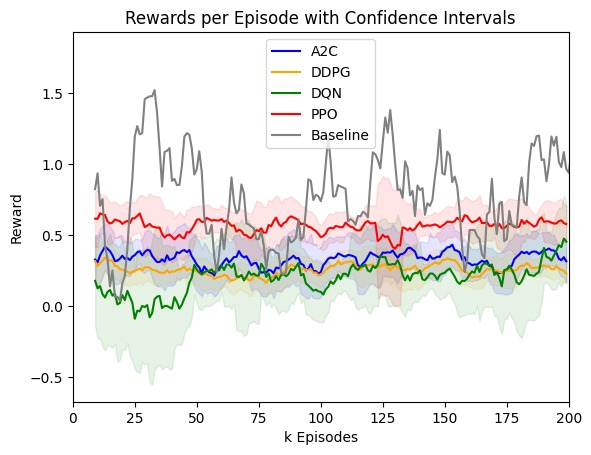
\includegraphics[width=\textwidth]{img/example1.jpeg}
	\caption{Belohnungen der unterschiedlichen Single-Agent-Verfahren pro Episode mit Konfidenzintervallen}
	\label{fig:bild1}
\end{figure}

\ref{fig:bild2} stellt einen Violin-Plot der Belohnungen der letzten 10.000 Episoden für die verschiedenen Agents dar und erlaubt so einen allgemeinen Vergleich der Stärke der unterschiedlichen Agents. Auch diese Grafik bestätigt die Erkenntnis, dass der \ac{PPO}-Algorithmus die besten Ergebnisse mit einem durchschnittlichen Score von 0,5 erzielen konnte. Es wird jedoch auch hier deutlich, dass, obwohl die Baseline-Methode deutlich höhere Schwankungen aufweist, diese weiterhin bessere Ergebnisse erreicht und eine durchschnittliche Belohnung von 0,7 erreicht.

\begin{figure}[h]
	\centering
	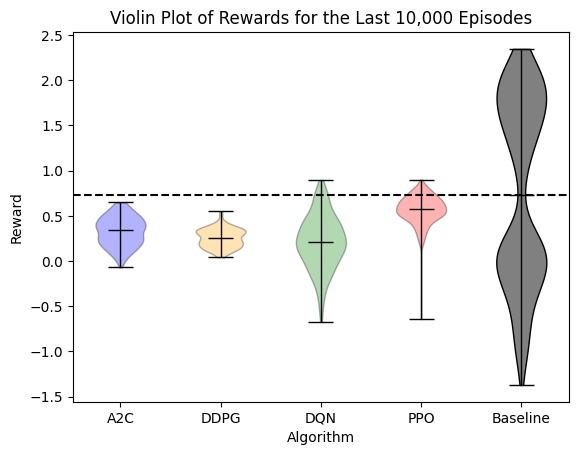
\includegraphics[width=\textwidth]{img/example2.jpeg}
	\caption{Violin-Plot der Belohnungen für die letzten 10.000 Episoden}
	\label{fig:bild2}
\end{figure}

Eine weitere einblicksreiche Betrachtung ist die Heatmap \ref{fig:todo}, welche die Bewegungen der Agents darstellen kann.

%MARL
Auch die Anwendung des \enquote{competitive-self play} Verfahrens für das Multi-Agent-Szenario wurde ausgewertet.

\fi


%todo: ggf. anmerken das wir ja schon eine ziemlich starke baseline entwickelt haben die auch anders als die agents information der umgebung nutzen kann